\documentclass[sigconf]{acmart}
\usepackage{booktabs}
\usepackage{listings}

\begin{document}

\title{Efficient MPI+OpenMP Programming with MPI 4.0}
\author{Dreßler Justus}
\orcid{0009-0005-0657-5854}
\affiliation{
    \institution{Friedrich Schiller University}
    \department{Faculty of Mathematics and Computer Science}
    \streetaddress{Fürstengraben 1, Main University Building (Universitätshauptgebäude)}
    \postcode{07743}
    \city{Jena}
    \country{Germany}
}
\email{justus.dressler@uni-jena.de}

\keywords{MPI, MPI+OpenMP,MPI+Threads}

\begin{CCSXML}
    <ccs2012>
    <concept>
    <concept_id>10010147.10010169</concept_id>
    <concept_desc>Computing methodologies~Parallel computing methodologies</concept_desc>
    <concept_significance>500</concept_significance>
    </concept>
    </ccs2012>
\end{CCSXML}

\ccsdesc[500]{Computing methodologies~Parallel computing methodologies}

\begin{abstract}

    Hybrid MPI+X programming is the current standard for High Performance Computing Applications.
    This paper focuses on how to write performant MPI+OpenMP programs.
    Parallelising with OpenMP and MPI together poses new challenges for efficient programs though.
    A main problem is communicating logical parallelism in the application to the MPI libraries like MPICH or OpenMPI.
    The new MPI 4.0 standard assists application developers with new hints and partitioned operations to simplify the exposure of that parallelism.
    This paper summarizes the operations that support fine grained parallelisation in current MPI 4.0, gives examples of how to apply them and gives recommendations based on the applications structure.


\end{abstract}

\maketitle

\section{Introduction}

Message Passing Interface (MPI) is the de facto standard for scaling High Performance Computing (HPC) Workloads across multiple compute nodes.
This paper will speak of MPI as the standard and refer to MPI implementations like MPICH and OpenMPI as "MPI libraries" going forward.
These MPI libraries implement the MPI standard while trying to achieve maximum performance.
To do so some libraries include extra library specific settings as hints, which the library user can set to increase possible performance.
Sometimes these libraries will also include entirely new ways to parallelize communication like MPIX\_Stream in MPICH \cite{Zhou2022}, but this paper will focus on methods in the MPI standard itself.

Traditionally applications relied on the memory-hungry MPI-Everywhere model \cite{zambreLessonsLearned2022}.
In the last decades however a rapid increase in core counts per CPU relative to other on-node resources necessitated a switch to a model of MPI+X,
where MPI is used to parallelize between different nodes and X is used to parallelize on each node.
Some popular choices for this second X part are CPU multithreading libraries like OpenMP or POSIX Threads, GPU Acceleration with CUDA or using MPI with Remote Memory Access calls for the communication within a node.
This paper will focus on MPI+OpenMP, though many aspects of this paper also apply for any other CPU multithreading library.

OpenMP is a popular library for generating shared-memory multithreaded programs.
It works under the fork join model, where a main thread does all the serial work and additional threads get spawned for multithreading when needed.
It is easy to add to existing serial code, mostly by adding comments called pragmas in front of loops.
Its ease of use also makes it popular for developing HPC software.
Currently MPI+OpenMP programs tend to perform worse than their MPI-Everywhere counterparts \cite{zambreLessonsLearned2022,zambreLogicalParallel2021}.
The main problem being extra unneeded thread synchronization overheads \cite{zambreLessonsLearned2022} and less exposure of parallelism for MPI libraries to use.

This paper gives an overview of ways to expose parallelism in communication to MPI libraries to achieve optimal performance (over 2x increase for communication-intensive programs \cite{zambreLogicalParallel2021}).
For this it will discuss mainly point-to-point communication. It compares traditional methods like generating multiple MPI communicators with the newer features of MPI 4.0, which introduced new hints to make tags a viable method of exposing parallelisation and added new partitioned operations which can gather contributions of multiple threads in parallel.

\section{Motivation}
The historically preferred method of MPI-Everywhere made logical parallelism easy to express in software.
It does however use up more memory and other on chip resources relative to MPI+OpenMP.
Classical MPI-Everywhere programs spawn a single process per core available while MPI+OpenMP programs normally only spawn a single process per node or NUMA domain \cite{zambreLessonsLearned2022}.

MPI point-to-point communication runs on so called communicators.
A MPI communicator defines which processes may talk with each other.
Each MPI process is required to keep a list of all participating MPI processes in the default communicator \verb|MPI_COMM_WORLD| \cite{mpi40}.
Assuming an $n$ core processor $n$ copies of the list are lying in each nodes memory in the MPI-Everywhere model.
An equivalent MPI+OpenMP program shares its list between its cores and also spawns $n$ times less processes, so \verb|MPI_COMM_WORLD| is $n$ times smaller and lies $n$ times less often in the memory of each processor.
For current generation processors exceeding 100 cores like Intel® Xeon® 6 \cite{intelXeon6} or 4th Generation AMD EPYC™ \cite{amd4thGenEpyc} this equates to a reduction of \verb|MPI_COMM_WORLD|'s memory consumption of over $n^2 > 10.000$ times.

Each MPI process also needs to be a full program, which means each core has to have all instructions duplicated.
OpenMP however only needs to generate code for the parallized parts (typically loops) of the program, which reduces the memory consumption for all additional cores significantly.

MPI+OpenMP programs do, however, tend to perform slower than MPI-Everywhere versions in practice \cite{zambreLessonsLearned2022}.
This is caused in part by accidental synchronization while calling the MPI library.
The MPI standard mandates a high amount of serialization to ensure correct communication, for example all messages on the same \verb|<Communicator,Rank>| pair are transmitted in non-overtaking order \cite{mpi40}.
This is important to prevent deadlocks (two processes each wait on the other) but also slows down the communication overall.
The rest of the paper dedicated to explain how such slowdowns may be prevented.
The paper will assume that \verb|MPI_INIT| has been called with \verb|MPI_THREAD_MULTIPLE| to enable multithreaded access to MPI \cite{mpi40}.

\section{Parallel Point-to-Point Communication in MPI 4.0}

Point-to-Point Communication refers to any communication between 2 different processes.
There are several ways to implement logical parallel point-to-point communication efficiently in MPI.
For MPI versions lower than 4.0 a unique communicators per logical parallel communication channel may be used.
MPI 4.0 introduced Partitioned Operations to aid efficient parallel communication.
In Partitioned Operations multiple threads each contribute a part of a larger message.
MPI 4.0 also added new hints, a way for a program to guarantee MPI that it will not use certain features, that can make tags viable for performant parallel communication.
Furthermore MPI 4.0 introduced MPI Sessions, which may be used for parallelization purposes, but are not considered in the scope of this paper \cite{MPISessions}.
In the following subsections this paper will discuss the mentioned methods in more detail.

\subsection{Communicator}

The simplest though maybe not most intuitive way to parallelize communication is to assign each logical parallel message its own communicator.
Since MPI implies no relative ordering on different communicators \cite{zambreLessonsLearned2022}, libraries can map messages on different communicators to different underlying message channels.
To use different communicator an MPI application developer needs to be aware of a few key problems:

\begin{figure}
    \caption{
        For ideal communication parallelism for 9 thread processes with a 3x3 grid that communicate along an axis, the left and right communicators on each process have to be distinct to avoid dependencies between left and right connections.
        Each unique colour represents a unique connector in the picture.
    }
    \Description[]{3x3 thread processes communicating along a single axis and the associated 3-point stencil oriented in parallelisation direction}
    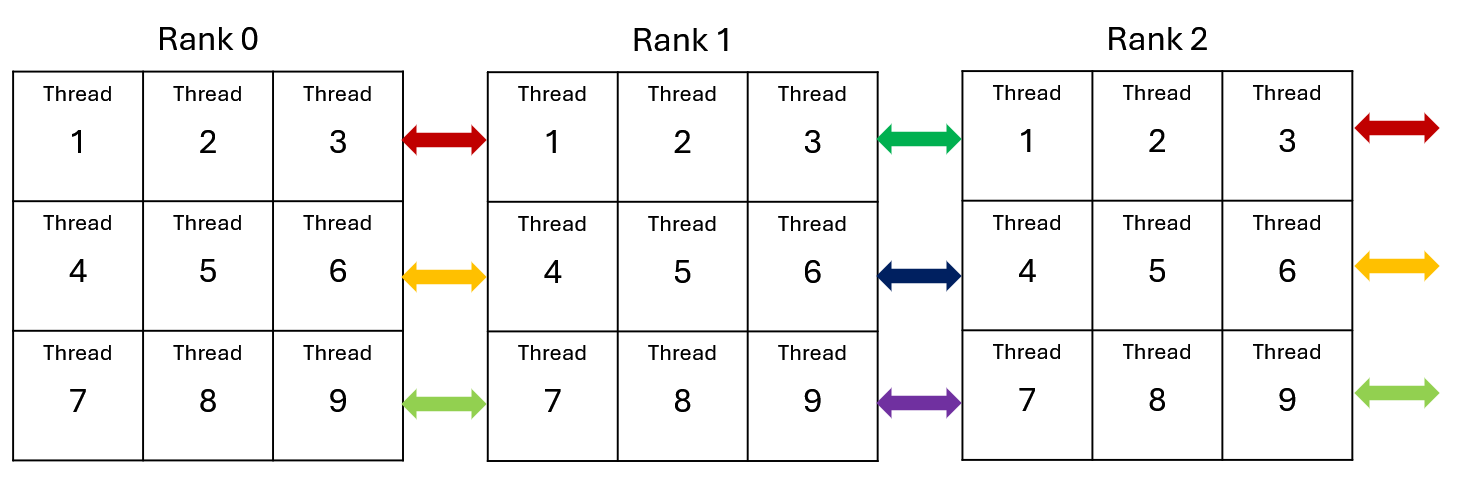
\includegraphics[width=0.47\textwidth]{Communicator_Line.png}
    \label{fig:Communicator_Line}
\end{figure}

\begin{figure}
    \caption{C++ implementation of Figure \ref{fig:Communicator_Line}}
    \Description[]{Code for 3x3 thread processes figure}
    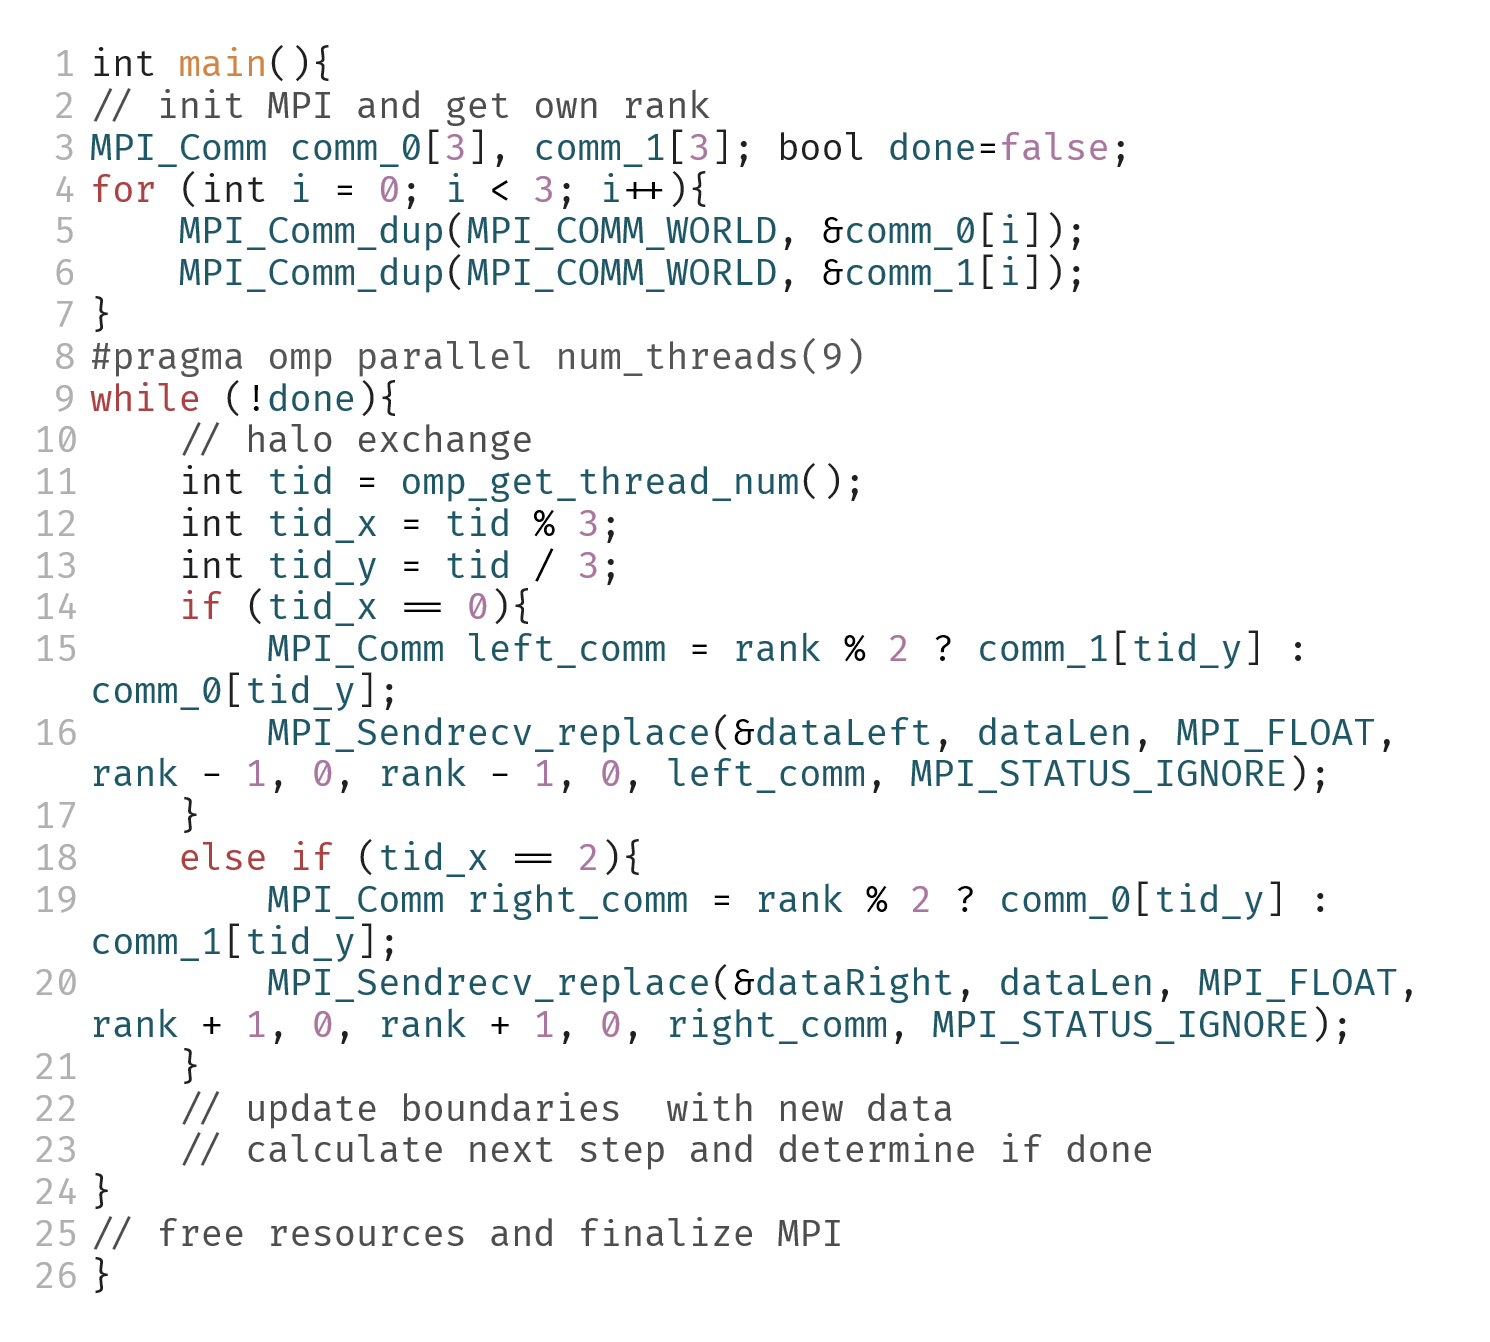
\includegraphics[width=0.47\textwidth]{Communicator_Line_CPP.png}
    \label{fig:Communicator_Line_CPP}
\end{figure}

\textbf{1)} \textit{For optimal parallelization there needs to be two communicator for each pair of threads communicating between different processes.}
To demonstrate the need for two communicators per pair of threads, imagine a problem where processes only need to communicate along a single axis as in Figure \ref{fig:Communicator_Line}.
If only one communicator is used per pair of threads, communication between \verb|<Rank_0,Thread_5>| and \verb|<Rank_1,Thread_3>| shares its communicator with the communication between \verb|<Rank_1,Thread_5>| and \verb|<Rank_2,Thread_3>|.
This is problematic since the messages from \verb|Rank_0| and \verb|Rank_2| to \verb|Rank_1| now run on the same communicator and the two exchanges are no longer independent.
A sample implementation can be seen in Figure \ref{fig:Communicator_Line_CPP}.

\textbf{2)} \textit{For large multidimensional stencils the number of communicators needed grows rapidly and an MPI program using those should consider other methods to expose parallelization.}
For more complex stencils like a 27-point 3D stencil as seen in Hypre\cite{hypre2020} on a 64-core processor (data distributed as [4,4,4] chunks) the number of communicators needed to expose all possible communication parallelism amounts to $6 \cdot 4^2$ for the sides plus $24 \cdot 4^2 - 8$ for the corner diagonal plus $24 \cdot 4^2 - 48$ for the edge diagonals, totalling $808$ communicators.
The workload would only need a single parallel communication channel for each thread communicating between nodes ideally though, which is only $4^3 - (4-2)^3 = 56$.
The equations were derived from those used by Zambre and Chandramowlishwaran \cite{zambreLessonsLearned2022}.
Generating so many communicators is not only complex, it also strains MPI libraries that have to map the many possibly parallel messages to a far smaller number of parallel paths in hardware, (as an example Omni-Path only has 160 hardware contexts \cite{intelOmniPath}).
Since the MPI library lacks the knowledge of the intended communication pattern its mapping to the relevant hardware contexts will be suboptimal.

\textbf{3)} \textit{Using communicators to expose parallelism and group processes introduces performance loss or limits the portability across MPI libraries.}
Since MPI 4.0 lacks standardised hints regarding communicator usage, MPI libraries cannot differentiate between communicators used to expose parallelism and those that are used for grouping processes together.
If a MPI library tries to parallelise across communicators, any communicator that is not used to expose parallelisation puts unnecessary strain on the library, reducing overall performance.
A MPI libary may provide extra hints to specify which communicators are used to expose parallelism, but using those makes the performance of the program depend on that library and makes swapping of libraries harder.

\begin{figure}
    \caption{processes with N worker and 1 main thread communicating irregularly; each worker thread needs to be able to communicate with all other main threads; Each coloured connection represents a unique communicator}
    \Description[]{3 Nodes with 1 main thread and N worker threads, from each worker thread there is a connection to all other main threads, each connection is coloured by the thread id of the worker thread}
    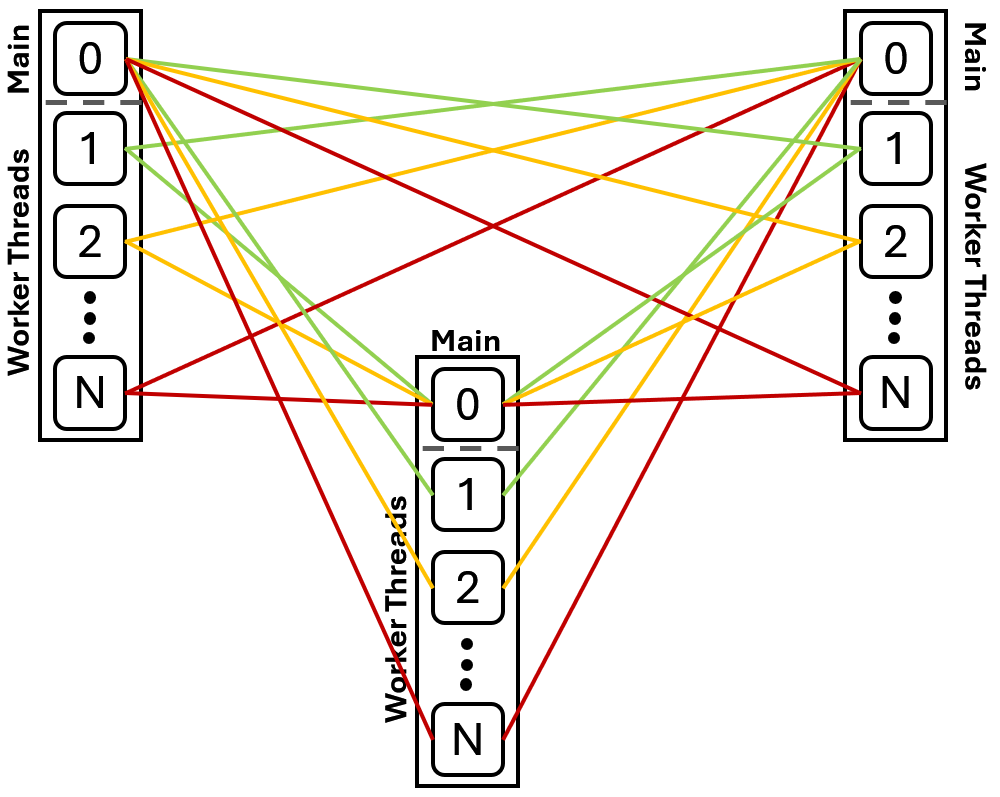
\includegraphics[width=0.47\textwidth]{Communicator_Irregular.png}
    \label{fig:Communicator_Irregular}
\end{figure}

\textbf{4)} \textit{Using communicators for irregular access patterns degrades performance.}
Imagine a task-based application with $n$ worker threads and one main thread in each process as depicted in Figure \ref{fig:Communicator_Irregular}.
All workers in one process may need to communicate with the main thread of any other process.
In such a case the software may either generate $n$ communicator for each worker thread in a process or generate $n \cdot m$ communicator for all $n$ worker in a process and all $m$ processes.
The latter version is infeasible for any non trivial number of processes as it generates way more communicators which strains the MPI library for the same reason large multidimensional stencils do.
So the software is realistically restricted to just $n$ communicators.
This then forces the main thread to communicate over the same communicators as its workers.
And as the main thread needs to iterate over all possible communicators it will contend with its workers to access the communicators and slow down the application.
This leads to communicators performing worse than other parallelisation alternatives.
As an example communicators performed 1.63x worse than tags with hints in the task-based framework Legion \cite{zambreLogicalParallel2021}.

\subsection{Tags with Hints}

MPI operations like \verb|MPI_SEND| take a \verb|<Rank,Tag,Communicator>| triple as input.
The tag is included to differentiate messages between the same processes on a single communicator.
Normally the MPI standard requires a non-overtaking order for all messages with the same \verb|<Rank,Communicator>| \cite{mpi40}.
So the default settings do not enable a program to use the additionally sent tags for parallelization.
If the program however guarantees MPI, that it will not use the \verb|MPI_ANY_TAG| (a parameter matching all tags), MPI libraries can send different messages between the same ranks but differing tags in arbitrary order.


\begin{figure}
    \caption{
        C++ Code to encode source and destination into a tag.
        The bitpattern of source and destination are simply appended at the left side of the tag.
    }
    \Description[]{Code to encode source and target into tag}
    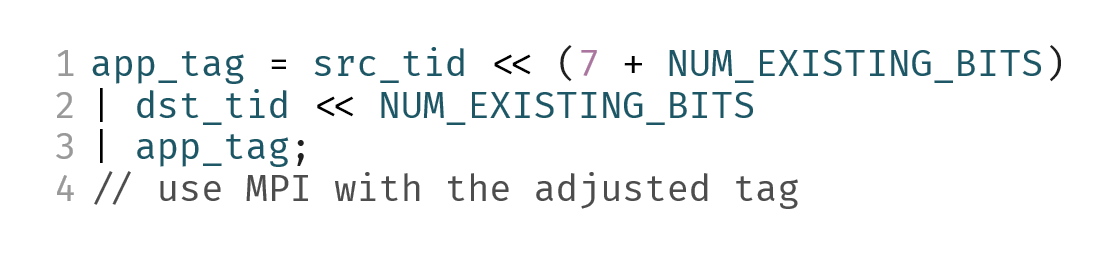
\includegraphics[width=0.47\textwidth]{Tags_CPP.png}
    \label{fig:Tags_CPP}
\end{figure}

To use this new avenue to expose parallelism, programs need to use the \verb|mpi_assert_no_any_tag| hint.
Now any MPI library is free to parallelize over different tags.
To use that a program can simply encode the source thread and target thread into the tag.
If the \verb|MPI_ANY_TAG| is needed for application logic, but the order of the operations getting matched is irrelevant, the program may instead use the \verb|mpi_assert_allow_overtaking| to ignore the non-overtaking behaviour completely on a communicator \cite{mpi40}.
A possible implementation is given in Figure \ref{fig:Tags_CPP}.
Using tags comes with some caveats:

As with communicators the other uses of tags may strain a library more than needed.
Libraries may include extra hints to help the mapping of tags to hardware channels, but using those hints binds the program performance to a specific library and makes swapping libraries harder.

Tags are restricted to 64 bits.
Depending on the programs other uses for tags this may be a non issue or a dealbreaker.
Encoding source and target thread in tags for $n$ core processors takes $2\log_2{n}$ bits.
For a 128 core processors this would mean, that a program reserves $2\log_2{128} = 14$ bits of their tags.
For most programs this will be irrelevant, but if the program already encodes much information in their tags, exposing parallelisation information additionally in tags might not be feasible.

\subsection{Partitioned Point-to-Point Communication}

\begin{figure}
    \caption{
        A C++ example of how to use partitioned operations with MPI.
        In the example 2 MPI processes do some calculation together, where the output of the first process gets consumed by the second process.
        There exists some synchronization to ensure only a single thread is able to call MPI\_Start and MPI\_Wait.
    }
    \Description[]{C++ Example Code for partitioned operations.}
    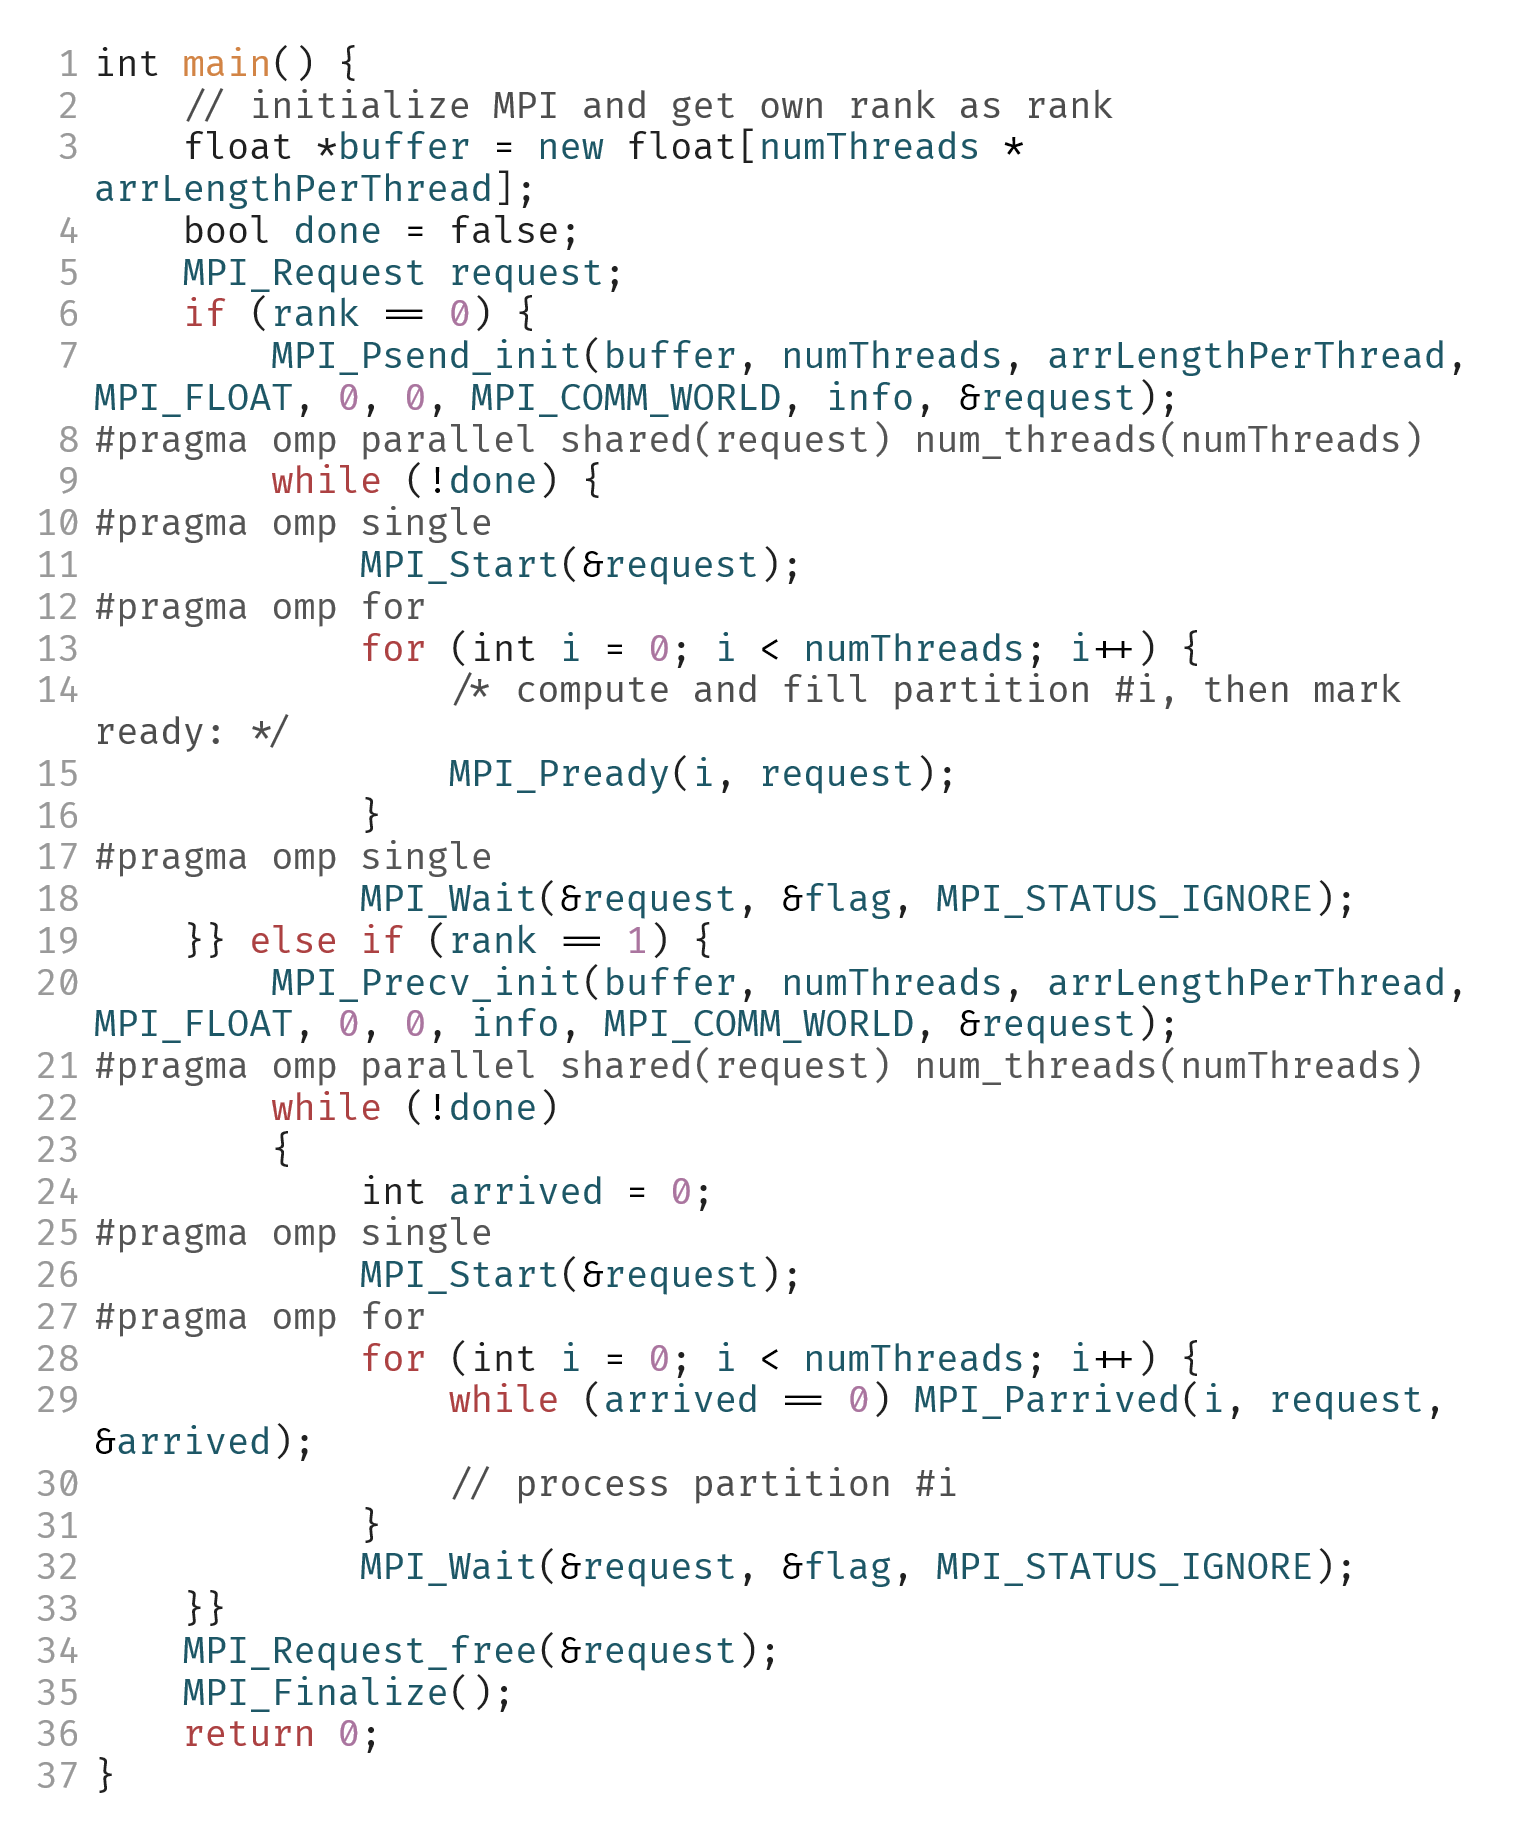
\includegraphics[width=0.47\textwidth]{PartitionOperations_CPP.png}
    \label{fig:PartitionedOps_CPP}
\end{figure}

Partitioned Operations are point-to-point operations where the message is partitioned into multiple parts.

To implement partitioned point-to-point operations is slightly more difficult than simple \verb|MPI_SEND| and \verb|MPI_RECV| calls.
In contrast to those all operations have to be first initialised on sender and receiver side with \verb|MPI_PSEND_INIT| and \verb|MPI_PRECV_INIT| respectively.
The initialisation may be done long before the operation is executed.
To start the execution there must be a single call to \verb|MPI_START|.
Then each contributing sending thread may write its part of the message in the shared buffer and then mark its part as ready by calling \verb|MPI_PREADY|.
On the receiving side threads may poll for completion of individual partitions of the message by calling \verb|MPI_PARRIVED|.
As soon as those return a truthy flag a thread may work on that partitions data.
There must be a single final call to \verb|MPI_WAIT| or \verb|MPI_TEST| to complete the operation, before it may be restarted with another call to \verb|MPI_START|.
An example of this can be seen in Figure \ref{fig:PartitionedOps_CPP}.

This more complicated setup allows a MPI library to transmit the partitions in parallel instead of waiting for all threads to finish working.
Partitioned operations are ideally suited to very regular communication, as found in stencil applications.
They are very ill suited for irregular communication though, as the operations have to be initialised before any communication may happen \cite{zambreLessonsLearned2022}.
Irregular communication is further complicated by the missing ability to provide wildcards (\verb|MPI_ANY_TAG|, \verb|MPI_ANY_SOURCE|) to \verb|MPI_PRECV_INIT| \cite{mpi40}, on which modern task-based runtimes like Legion rely \cite{zambreLessonsLearned2022}.


\section{Parallel Remote Memory Access in MPI 4.0}

\begin{figure}
    \caption{
        A C++ example of how to create a MPI\_Window, that does not enforce ordering for MPI\_Accumulate operations.
    }
    \Description[]{C++ Example Code to create a MPI_Window without ordering on accumulate}
    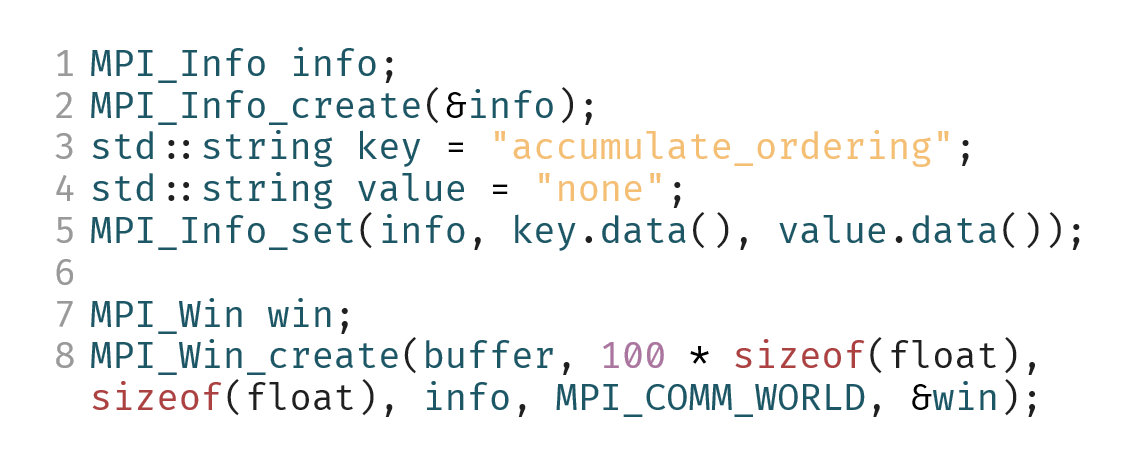
\includegraphics[width=0.47\textwidth]{RMANoOrdering.png}
    \label{fig:RMANoOrdering_CPP}
\end{figure}

Remote Memory Accesses (RMA) are one sided communications, where the target does not need to do anything after the initialisation.
Those operations are only allowed on specific sections of their memory called windows in MPI.
To create such a window, all processes in a communicator have to call \verb|MPI_WIN_CREATE|.
They may specify different memory sizes for their window, including specifying \verb|size=0| to not expose any memory themselves.
In those windows other processes may put data with \verb|MPI_PUT| or get data from with \verb|MPI_GET| or their non-blocking alternatives \cite{mpi40}.
These RMA operations are not matched on the destination, hence being called one-sided.
In contrast to point-to-point communication MPI imposes no order requirement for \verb|MPI_PUT| and \verb|MPI_GET| operations \cite{mpi40}.
So for these operations MPI libraries are free to parallelize them as needed.
MPI windows also allow atomic \verb|MPI_ACCUMULATE| operations.
This operation updates a target value by adding a number to it atomically.
MPI imposes strict ordering on \verb|MPI_ACCUMULATE| operations per default.
If such a ordering guarantee is not needed, Zambre and Chandramowlishwaran list NWChem as such an example \cite{zambreLessonsLearned2022}, it may be relaxed on window creation by specifying another \verb|accumulate_ordering|.
The MPI standard supports specifying no ordering or only a subset of read-after-read, read-after-write, write-after-read, write-after-write in such a case \cite{mpi40}.
An example of no ordering can be seen in Figure \ref{fig:RMANoOrdering_CPP}.

\section{Conclusions}

In this paper I demonstrate multiple ways to expose communication parallelism to MPI libraries in MPI 4.0 while using CPU multithreading.
It has been demonstrated that communication can be a significant bottleneck and exposing available parallelism to MPI libraries increase performance by over 2x for some applications \cite{zambreLogicalParallel2021}.
From the described methods I would recommend tags with hints if the application does not rely on the \verb|MPI_ANY_TAG|.
It is the easiest to include into existing applications and performs no worse than its alternatives \cite{zambreLessonsLearned2022}.
Any of the described methods will work for most application types though.


\bibliographystyle{ACM-Reference-Format}
\bibliography{citations}

\end{document}
